% !TEX program = xelatex
% 2026 年度“策联杯”数学建模精英联赛 B 题参赛论文
\documentclass[zihao=-4,a4paper]{ctexart}

\usepackage[top=2.5cm,bottom=2.5cm,left=2.5cm,right=2.5cm]{geometry}
\usepackage{amsmath,amssymb,amsfonts,bm}
\usepackage{graphicx}
\usepackage{booktabs}
\usepackage{array}
\usepackage{caption}
\usepackage{float}
\usepackage{enumitem}
\usepackage{multirow}
\usepackage{makecell}
\usepackage{fancyhdr}
\usepackage{listings}
\usepackage{xcolor}
\usepackage[hidelinks]{hyperref}

% 图片路径
\graphicspath{{../output/}}

% 页码：页脚中部，从摘要页开始编号
\pagestyle{fancy}
\fancyhf{}
\fancyfoot[C]{\thepage}
\renewcommand{\headrulewidth}{0pt}
\setcounter{page}{1}

% 代码/伪代码样式
\definecolor{codebg}{RGB}{247,247,247}
\lstset{
  basicstyle=\ttfamily\footnotesize,
  backgroundcolor=\color{codebg},
  frame=single,
  rulecolor=\color{gray!40},
  breaklines=true,
  keywordstyle=\bfseries,
  commentstyle=\color{gray},
  tabsize=2,
  columns=fullflexible,
}

\captionsetup{font=small,labelsep=quad}
\setlength{\parindent}{2em}

\title{海上油田人员直升机运载计划编排}
\author{}
\date{}

\begin{document}

%==================== 摘要页（第 1 页）====================
\begin{center}
  {\LARGE\bfseries 海上油田人员直升机运载计划编排}\\[1.5em]
  {\Large\bfseries 摘\quad 要}
\end{center}
\vspace{0.8em}

海上油田生产连续、人员倒班集中，需以直升机承担出海、海返与穿梭三类人员运输。本文针对 3 座陆地机场、52 座海上设施、三种机型与 8 座可加油设施构成的运载系统，在最小化总飞机使用时间的基础上兼顾人员总在途时间、座位利用率与油耗等次要因素，建立了随问题递进的三个模型，并以精确算法求解。

\textbf{针对问题一}（单向出海运输，1600 人），本文将其抽象为多机场、多机型、带容量与燃油约束的单向车辆路径问题（CVRP 变体）。利用需求按设施编号自然分块、架次不跨机场中转与飞机充足三条结构性事实，把问题按机场解耦为三个同构子问题；对单机场子问题采用"机型感知拆分 + 集合划分"模型，将每设施需求拆为"满座份 + 尾数份"，满座份满载单飞、尾数份合并为环游，并以显式枚举 + 整数规划精确求解，燃油约束简化为"相邻加油点间累计距离不超过最大不加油航程"的可行性规则。结果表明，总飞机使用时间 \textbf{15061} 分钟、人员总在途时间 \textbf{131033} 分钟、总架次数 \textbf{88}、总燃油消耗量 \textbf{120920.1} kg、座位利用率 \textbf{49.68\%}；以 85 架次为理论架次数下界，LP 松弛下界 15041 分钟，求解 gap 为 \textbf{0.13\%}。

\textbf{针对问题二}（出海、海返与穿梭联合运输，4000 人），本文将其升级为带同时取送的车辆路径问题（VRPSPD）。核心发现是出海与海返在设施层面高度配对（净差落在 $[-4,+6]$），据此提出"配对往返、穿梭顺路承载"的建模思路：满座部分配对为往返架次使架次数近乎减半，尾数由出海、海返独立合并为环游，穿梭作为环游途中顺路承载的部分承载量；建立以 OD 对为覆盖对象的集合划分整数规划，目标分层加权（第一层最小化总飞机使用时间，第二层在航时最优解集内对油耗与座位利用率加权取优），并以 DFS 定价子问题的列生成精确求解。结果表明，总飞机使用时间 XXX 分钟、人员总在途时间 XXX 分钟、总架次数 XXX、总燃油消耗量 XXX kg、座位利用率 XX\%。

\textbf{针对问题三}（带时间要求的多日排班，4000 人 + 24 架飞机），本文在 VRPSPD 之上叠加时间窗与有限机队两重约束。核心发现是任务类型与窗口紧度高度相关：应急处置与增储上产共 400 人窗口落在单天之内、被锁定在窗日且只能小群组直飞，常规倒班与临时任务共 3600 人窗口跨 2--4 天、"哪天飞"成为决策变量，据此提出"紧核单天固定、松壳跨天可选"的分层思路。建立"日级主问题 + 天内排班"两层模型：日级主问题把集合划分列生成推广为"航线 + 执行日"候选列，仅以"总覆盖 + 逐日计数 + 日容量"三条约束精确刻画日指派；天内排班以时间索引整数规划把每日架次排到 8 架飞机时间轴上；临时任务按两阶段处理（先排非临时得总时间上界，再在上界内最大化临时满足人数），目标分层加权。结果表明，临时人员满足 XXX 人（满足率 XX\%），总飞机使用时间 XXX 分钟、人员总在途时间 XXX 分钟、总架次数 XXX、总燃油消耗量 XXX kg、座位利用率 XX\%。

\vspace{1em}
\noindent\textbf{关键词：}直升机运载计划；车辆路径问题；集合划分；列生成；分层规划；整数规划

\newpage

%==================== 一、问题重述 ====================
\section{问题重述}

海上油田由多个油气田及配套生产设施构成，生产运行、安全管理、设备维修与后勤保障等环节需要不同专业人员长期驻守，海岗员工到期后集中换班。换班时接班人员出海、离岗人员海返，生产任务与检维修安排还会带来设施之间的穿梭，人员往返主要由直升机运输。本题聚焦这一人员运输系统，包含 3 座陆地机场（A01、A02、A03）与 52 座海上设施（F001--F052），海上设施均位于距海岸 100--250 km 海域，其中 8 座（F006、F011、F018、F024、F031、F038、F044、F050）设有可加油点。人员运输按业务性质分为应急处置、增储上产、常规倒班、临时任务四类，优先级依次递减；将人员自陆地机场送往海上设施称为\textbf{出海}、自设施返回机场称为\textbf{海返}、自一座设施前往另一座称为\textbf{穿梭}。

可用的直升机机型为 T1、T2、T3，主要参数见表~\ref{tab:aircraft}。每个架次从机场满油起飞，到达每一处地点以及最终返回机场时的剩余燃油不得低于该机型最低安全余油量，停靠期间不另计油耗；在可加油设施停靠时可选择是否加油，加油即加满，不加油每次停靠至少 10 分钟、加油至少 20 分钟。不考虑机场、设施与加油站的并发容量限制。

\begin{table}[H]
  \centering
  \caption{三种直升机的主要参数}
  \label{tab:aircraft}
  \begin{tabular}{cccccc}
    \toprule
    机型 & 座位数 & 速度 (km/h) & 油耗 (kg/km) & 油箱容量 (kg) & 最低安全余油量 (kg) \\
    \midrule
    T1 & 12 & 250 & 3.4 & 1000 & 150 \\
    T2 & 16 & 220 & 2.5 & 1150 & 150 \\
    T3 & 19 & 190 & 2.9 & 1600 & 200 \\
    \bottomrule
  \end{tabular}
\end{table}

本题的考核目标是\textbf{飞机使用时间}，即一个架次自机场起飞至返回同一机场的时间、含飞行与海上停靠，总飞机使用时间为各架次之和；同时需考虑\textbf{人员总在途时间}与\textbf{座位利用率}两项次要因素，前者指人员自其所乘飞机离开起点至到达终点的总时长，后者指全部航段客座公里与可用座公里之比。需完成以下三个问题：

\textbf{问题 1：单向出海运输。}peopleQ1.csv 给出 1600 条出海需求，不考虑时间窗与业务优先级、飞机数量充足，在最小化总飞机使用时间的基础上尽可能优化座位利用率、油耗等次要因素，输出 q1-routes.csv 与 q1-assignments.csv，并报告总飞机使用时间、人员总在途时间、总架次数、总燃油消耗量、座位利用率五项指标。

\textbf{问题 2：出海、海返与穿梭联合运输。}peopleQ2.csv 给出 4000 条出海、海返与穿梭需求，同样不考虑时间窗与优先级、飞机充足，在最小化总飞机使用时间的基础上尽可能优化其他因素，输出 q2-routes.csv 与 q2-assignments.csv，并报告五项指标。

\textbf{问题 3：带时间要求的多日排班。}peopleQ3.csv 在问题 2 基础上为每名人员增加最早登机时刻、最晚到达时刻与任务类型，需求时间落在 2026-08-03 至 08-10 之间。使用表~\ref{tab:fleet} 所列 24 架飞机，机场运营时段内可在 06:00--18:00 起飞、不得晚于 20:00 返回、不得在海上过夜，同一飞机完成一个架次后至少经过 30 分钟机场周转。临时任务可因减少开销而取消：先在不考虑临时任务时编排得到总飞机使用时间，再在不超过该时间的条件下尽可能多地满足临时需求，输出 q3-routes.csv 与 q3-assignments.csv，并报告临时满足情况与五项指标。

\begin{table}[H]
  \centering
  \caption{排班可用直升机（表 3）}
  \label{tab:fleet}
  \begin{tabular}{ccccc}
    \toprule
    机场 & T1 & T2 & T3 & 合计 \\
    \midrule
    A01 & 3 & 3 & 2 & 8 \\
    A02 & 2 & 4 & 2 & 8 \\
    A03 & 2 & 3 & 3 & 8 \\
    \midrule
    合计 & 7 & 10 & 7 & 24 \\
    \bottomrule
  \end{tabular}
\end{table}

%==================== 二、问题分析 ====================
\section{问题分析}

三个问题构成一条由简到繁、逐层递进的建模链，其本质是同一运输系统在不同约束维度下的车辆路径问题（VRP）变体：

\begin{enumerate}[itemsep=2pt]
  \item \textbf{问题一}：只有出海单向运输、人员只下不上，是带容量与燃油约束的单向 CVRP；
  \item \textbf{问题二}：加入海返与穿梭，同一架次既承载出海的到达又承载海返的出发，机上人数沿环游先减后增、不再单调，且每名人员须由同一架次直送终点、不得换乘，升级为带同时取送的 VRPSPD；
  \item \textbf{问题三}：在问题二路由结构不变的基础上，叠加时间窗与有限机队两重约束，是 VRPTW 与机队调度的结合。
\end{enumerate}

我们的建模沿同一主线展开：先观察数据、找出结构性特征，再据此分解问题、构造候选解，最后选择规模上可行、质量上可评估的算法。沿这条主线，我们观察到四点关键性结构特征，它们决定了后续全部的建模与求解路径：

\textbf{（1）三机场严格解耦。}我们发现指定机场的人员天然落在其所属设施号段——A01 服务 F001--F017、A02 服务 F018--F035、A03 服务 F036--F052；穿梭 OD 全部位于同一区块内，跨机场人数为 0。再结合架次不跨机场中转，以及问题一、二中飞机充足、问题三中机队按机场固定的题设，于是按设施分块即可把总问题分解为三个互不相干的子问题，且不损失任何最优性。

\textbf{（2）"满座 + 尾数"需求拆分。}单机最多 19 座而每设施需求 19--51 人，任一设施的需求都须拆分给多个架次共同运送。既然满载直飞已是这部分人员最快的运送方式，我们就把每设施需求拆成"满座份 + 尾数份"：满座份满载单飞、直接固化为成本；尾数份，也就是拆不尽的剩余人数，跨设施合并为环游、一次飞多设施以省去多次机场往返。这样优化空间就被压缩到"尾数合并"这一个环节，而合并只受座位数不超过 19 与停靠次数不超过 5 的双重约束。

\textbf{（3）出海与海返高度配对。}对问题二数据的预分析显示，各设施出海与海返人数之差落在 $[-4,+6]$、48/52 个设施在 $\pm3$ 以内，即"送去多少人、几乎接回多少人"。受此启发，我们把满座部分配对为往返架次，去程满载送达、返程满载接回，一个架次兼负两程、使架次数近乎减半；只有真正新增的穿梭客流与未配对的少量尾数需要额外运力。

\textbf{（4）任务类型与窗口紧度高度相关。}对问题三数据的预分析发现，应急处置与增储上产共 400 人的窗口全部落在单天之内，最短者不足半小时，其航班被迫落在窗日、只能小群组直飞；常规倒班与临时任务共 3600 人的窗口跨 2--4 天，"哪天飞"才是真正的决策变量。据此我们把需求分为\textbf{紧核 400 人}与\textbf{松壳 3600 人}两层，前者单天固定、后者跨天可选，其求解顺序恰与题目"应急处置 $\to$ 增储上产 $\to$ 常规倒班 $\to$ 临时任务"的优先级一致。

四点特征依次对应后文的四个关键决策：特征 (1)(2) 支撑问题一的"解耦 + 拆分 + 精确求解"；特征 (3) 让问题二只需在问题一框架上新增海返与穿梭两类客流，但把求解算法从显式枚举升级为列生成；特征 (4) 决定问题三"日级主问题 + 天内排班"的两层结构与两阶段编排。

%==================== 三、模型假设 ====================
\section{模型假设}

\begin{enumerate}[itemsep=2pt]
  \item 因题面未给出人员上下机与地面调度时间，故将其忽略不计，仅计飞行时间与海上停靠时间；
  \item 题面给定飞行速度与单位距离油耗不随载客量变化，满载与空载航速、油耗相同；
  \item 题面给定机场、海上设施与加油站的并发容量无需考虑，故忽略其限制；
  \item 停靠时间取最小值：不加油 10 分钟、加油 20 分钟，允许等待延长；所有时间向上取整到整数分钟；
  \item 距离矩阵对称且满足三角不等式，可直接用于 TSP 求解；
  \item 题面要求每名人员由同一架次自起点直送终点、中途不得换乘；
  \item 架次自某机场起飞、最终返回同一机场，不跨机场中转。
\end{enumerate}

%==================== 四、符号说明 ====================
\section{符号说明}

\begin{table}[H]
  \centering
  \caption{主要符号说明}
  \label{tab:notation}
  \small
  \begin{tabular}{ll}
    \toprule
    符号 & 含义 \\
    \midrule
    $\mathcal{A}=\{A01,A02,A03\}$ & 机场集合 \\
    $\mathcal{F}=\{F001,\dots,F052\}$ & 海上设施集合，$|\mathcal{F}|=52$ \\
    $\mathcal{R}\subset\mathcal{F}$ & 可加油设施集合（8 个） \\
    $\mathcal{M}=\{T1,T2,T3\}$ & 机型集合 \\
    $\mathcal{D}=\{1,\dots,7\}$ & 规划期天数集合（问题三） \\
    $\mathcal{T}$ & 任务类型集合（问题三） \\
    $c_m, v_m, f_m, U_m, \underline{u}_m$ & 机型 $m$ 的座位数、速度、油耗、油箱容量、最低安全余油量 \\
    $\bar d_m=(U_m-\underline{u}_m)/f_m$ & 机型 $m$ 的最大不加油航程 \\
    $d_{uv}$ & 节点 $u,v$ 间距离（km） \\
    $q_d^{\text{out}}, q_d^{\text{ret}}, q^{\text{sh}}_{(i,j)}$ & 设施 $d$ 出海、海返人数及穿梭 OD $(i,j)$ 人数 \\
    $D_{(i,j)}^{\tau}$ & OD $(i,j)$ 上任务类型 $\tau$ 的需求人数（问题三） \\
    $r$、$a_r$、$m_r$、$S_r$ & 架次（列）及其起飞机场、机型、访问设施子集 \\
    $d_r^{\text{TSP}}$、$T_r$、$k$、$g_r$ & 架次 $r$ 的环游距离、总时间、海上停靠次数、加油次数 \\
    $n_{r,(i,j)}$ & 架次 $r$ 承载 OD $(i,j)$ 的人数 \\
    $\lambda_r$（$\lambda_{r,d}$） & 架次 $r$（第 $d$ 天）的使用次数（整数变量） \\
    $y_s$、$n_s$、$p_s$ & 拆分方案 $s$ 的选择变量、满座份数、尾数份人数（问题一） \\
    $P_r, F_r, E_r$ & 架次 $r$ 的人员总在途时间、油耗、空座$\cdot$距离（次指标系数） \\
    $P_0,F_0,E_0$；$w_P,w_F,w_\eta$ & 无量纲化基准；次指标权重（$w_P+w_F+w_\eta=1$） \\
    $\eta$ & 座位利用率 \\
    $z_{LP}, z_{IP}$ & 集合划分 IP 的 LP 松弛下界、整数最优值 \\
    \bottomrule
  \end{tabular}
\end{table}

%==================== 五、问题一 ====================
\section{问题一：单向出海运输的直升机运载计划编排}

\subsection{三机场解耦与单机场子问题的建立}

问题一需同时决定每名乘客的起飞机场、每架次访问的设施集合与顺序、机型以及加油方案，规模大且 NP-hard，直接整体求解不可行。我们转而寻找可分性，观察到三条结构性事实：人员不可换乘、架次不跨机场中转、飞机数量充足。由前两条，任一架次自始至终只服务其起飞机场周边的设施；由第三条，机场间无需共享资源。故\textbf{只要每名乘客的起飞机场被确定，总问题即退化为三个互不相干、结构完全相同的单机场子问题}：

\begin{equation}
  \min \sum_{a\in\mathcal{A}} \mathrm{VSP}(a)
\end{equation}

其中 $\mathrm{VSP}(a)$ 为机场 $a$ 的单机场航线编排子问题。唯一障碍是 1353 名 LAND 乘客没有指定起飞机场，若把机场选择留作决策变量，三机场将通过 LAND 乘客相互耦合。因此，下一小节借助"设施沿海岸线线性排列、编号与机场位置一致"的地理结构，把 LAND 乘客按设施分块固定归属机场，从而把机场选择退化为固定参数，完成分解。

\subsection{LAND 乘客的机场归属与三机场解耦}

设施编号 F001--F052 沿海岸线自北向南线性排列，与三机场位置分布一致，故按编号等分为三段即可同时兼顾"就近"与"均衡"：

\begin{equation}
  \sigma(d)=\begin{cases}
    A01, & d\in\{F001,\dots,F017\}\\
    A02, & d\in\{F018,\dots,F035\}\\
    A03, & d\in\{F036,\dots,F052\}
  \end{cases}
\end{equation}

三段负载分别为 499/598/503 人，接近均衡。将设施 $d$ 的全部需求统一由 $\sigma(d)$ 服务，则各机场的设施集合与人数均为固定参数 $\mathcal{F}_a=\{d:\sigma(d)=a\}$、$q_{d,a}=q_d\,\mathbb{1}[\sigma(d)=a]$。由数据统计，指定机场乘客的分布与式~(2) 的分块完全一致，故 $\sigma(d)$ 对所有乘客都是其天然归属。这一步以放弃"设施分给非所属机场"为代价，换取子问题规模的大幅下降——该代价对指定机场乘客为零，因其分布与分块完全一致；对 LAND 乘客则仅是一种近似，其合理性在 §8 的改进中进一步讨论。

\subsection{单机场的架次编排模型}

固定一个机场 $a$，其设施人数记为 $q_d$。模型沿"先拆分、再合并、后选择"的思路分四步：需求拆分为"满座份 + 尾数份"，满座份固化为成本，尾数份合并为环游，最后用集合划分 IP 统一选择。拆分的思想直接来自结构特征 (2)——满载直飞已是最快的运送方式，真正需要决策的只是拆不尽的尾数。

\subsubsection{超容量设施需求的多机型拆分}

同一设施的需求可能由任一机型运送，且拆分方式决定后续尾数合并的空间。因此我们干脆把"机型 $\times$ 拆分方式"的每种可能都生成一个候选拆分方案 $s=(m_s,n_s,p_s)$，把机型选择与拆分的耦合交给最终 IP 择优：

\begin{equation}
  n_s=\left\lfloor\frac{q_d}{c_{m_s}}\right\rfloor,\qquad p_s=q_d-c_{m_s}\,n_s
\end{equation}

其中 $n_s$ 为满座架次数、每架满载 $c_{m_s}$ 人，$p_s$ 为拆不尽的尾数份人数且 $0\le p_s<c_{m_s}$。例如 $q_d=29$：T3 得 $(19,1,10)$、T2 得 $(16,1,13)$、T1 得 $(12,2,5)$，三种方案构成候选集合 $D_d$，机型选择与需求拆分在此耦合、由 IP 择优。

\subsubsection{满载份的独立运送与固定时间成本}

满座份人数恰等于座位数，满载单飞已是该部分人员的最快运送方式，再并入其他设施只会增加飞行与停靠，故满座架次不参与合并、直接固化为固定成本：

\begin{equation}
  T^{\text{满}}(d,m)=\frac{2\,d_{\sigma(d),d}}{v_m}+10+10\,g
\end{equation}

其中 $g\in\{0,1\}$ 表示该满座架次是否加油，由燃油判据确定；若该机型无法直达，即往返超过最大不加油航程且 $d$ 非可加油设施，则此方案剔除。

\subsubsection{尾数份的跨设施合并运送}

真正需要决策的只剩各设施的尾数份。以 $(d,m_s)$ 标识一条尾数份，即设施 $d$ 在机型 $m_s$ 下的尾数、人数 $p_s$，于是一个架次可把若干不同设施的尾数份合并为一条"机场 $\to$ 若干设施 $\to$ 机场"的环游。设尾数合并架次 $r$ 含尾数份集合 $\Theta_r$、访问设施集合 $S_r$、机型 $m_r$，须满足

\begin{equation}
  \sum_{(d,m_s)\in\Theta_r} p_s \le c_{m_r},\qquad |S_r|\le 5
\end{equation}

即总人数不超过座位数、海上停靠不超过 5 次，且同一设施至多出现一条尾数份。其成本为

\begin{equation}
  T_r=\frac{d_r^{\text{TSP}}}{v_{m_r}}+10\,|S_r|+10\,g_r
\end{equation}

其中 $d_r^{\text{TSP}}$ 为访问 $S_r$ 中设施的最短环游距离，由不超过 5 个点的 TSP 求得。

\subsubsection{覆盖全部需求的架次选择整数规划}

之所以选择集合划分而非逐弧流模型，是因为拆分与合并后的候选架次数有限、仅有数千至数万，如 §5.6 所析，可全部显式枚举，且每条架次的耗时、油耗可预先精确核算、直接对应输出文件中的一条航线，IP 只需回答"选哪些"。为此为每个拆分方案设 0-1 变量 $y_s$、为每条尾数合并架次设整数变量 $\lambda_r$，得集合划分 IP：

\begin{equation}
  \min \sum_{d}\sum_{s\in D_d} y_s\,n_s\,T^{\text{满}}(d,m_s)+\sum_{r}T_r\,\lambda_r
\end{equation}

\begin{equation}
  \text{s.t.}\quad \sum_{s\in D_d} y_s=1,\quad \forall d\in\mathcal{F}_a
\end{equation}

\begin{equation}
  \sum_{r:\ (d,m_s)\in\Theta_r}\lambda_r = y_s,\quad \forall d,\ \forall s\in D_d,\ p_s>0
\end{equation}

\begin{equation}
  y_s\in\{0,1\},\qquad \lambda_r\in\mathbb{Z}_+
\end{equation}

式~(7) 第一项为满座架次固定时间、第二项为尾数合并架次时间；式~(8) 保证每设施恰选一个拆分方案；式~(9) 把所选方案的尾数份与其运载架次对齐。容量与停靠上限已内化于列定义（式~(5)），无需在 IP 中显式写出。

\subsection{最小化总航时并兼顾次指标的分层目标}

题目要求"在最小化总飞机使用时间的基础上尽可能优化次要因素"——这是一个典型的分层结构，即字典序结构：主目标优先，次要因素只在主目标最优的解集内起区分作用。据此三问统一采用\textbf{分层加权}目标：第一层最小化总飞机使用时间，对应式~(7)；第二层在航时最优解集内对油耗与座位利用率加权取优。设第一层最优航时 $T^*$，第二层为

\begin{equation}
  \min\ \Big[w_F\frac{F}{F_0}+w_\eta\frac{E}{E_0}\Big]
  \qquad\text{s.t.}\quad \sum_{d,s}y_s n_s T^{\text{满}}(d,m_s)+\sum_r T_r\lambda_r=T^*,\quad \text{式}(8)\text{--}(10)
\end{equation}

其中 $F$、$E$ 为总油耗与总空座$\cdot$距离，空座$\cdot$距离是座位利用率的线性代理；$F_0,E_0$ 为无量纲化基准，权重 $w_F+w_\eta=1$ 由层次分析法确定并经敏感性分析验证。由于问题一架次结构由容量与燃油约束主导、尾数合并自由度有限，第二层次指标对总航时的影响极小，故以第一层最优解报告各项指标。

\subsection{架次燃油可行性与中途加油点插入}

燃油约束是航线的可行性条件而非目标项：要求每架次全程剩余油量不低于安全余油。若逐弧跟踪油量，每条候选架次都要引入连续变量、使 IP 显著膨胀；而下面的递推显示，由于"加油即加满"，油量约束具有局部结构，可退化为对候选列的简单校验。记架次路线为 $a=s_0\to s_1\to\cdots\to s_k\to s_{k+1}=a$，飞机满油起飞，到达每站后剩余油量递推：

\begin{equation}
  u_i=\begin{cases}
    U_m, & s_i\in\mathcal{R}\ \text{且在该站加油}\\
    u_{i-1}-f_m\,d_{s_{i-1},s_i}, & \text{否则}
  \end{cases}
\end{equation}

可行性要求每一站以及返回机场处 $u_i\ge\underline{u}_m$。由于加油即加满，式~(12) 等价于：\textbf{任意两个相邻加油点以及起降机场之间的累计飞行距离不超过最大不加油航程 $\bar d_m$}。三种机型 $\bar d_{T1}=250$、$\bar d_{T2}=400$、$\bar d_{T3}\approx483$ km；A03 南端的 F037--F052 距机场 243--403 km、往返超 T3 航程，必须利用可加油设施中途加油。因此，对超航程架次，在其间就近插入 $\mathcal{R}$ 加油点即可修复。

\subsection{单机场子问题的精确求解与解质量评估}

解耦后每机场仅 17--18 个设施，我们的首选是显式枚举：只要候选架次能全部列出，集合划分 IP 即可直接精确求解、无需任何启发式。下面的枚举量分析支持这一选择，故采用"显式枚举候选 + 集合划分整数规划"精确求解，流程为：\textbf{(1)} 生成拆分候选与满座架次；\textbf{(2)} 深度优先回溯枚举尾数合并架次，剪枝条件为累计人数不超过 19、停靠不超过 5、同一设施至多一条尾数份；\textbf{(3)} 构建并求解集合划分 IP，由 CBC 精确求解；\textbf{(4)} 燃油逐列校验与加油点插入修复；\textbf{(5)} 以 LP 松弛下界评估解质量。

以拥有 17 座设施的 A01 为例，尾数合并组合数上界为 $\sum_{k=1}^{5}\binom{17}{k}3^k\approx1.7\times10^6$，经"人数 $\le19$"剪枝后实际列数仅数千至数万，完全可枚举。

\subsection{问题一的求解结果与指标分析}

\begin{table}[H]
  \centering
  \caption{问题一五项指标与解质量}
  \label{tab:q1res}
  \begin{tabular}{lcc}
    \toprule
    指标 & 数值 & 说明 \\
    \midrule
    总飞机使用时间 & 15061 min（251.0 h） & 主目标 \\
    人员总在途时间 & 131033 min（2183.9 h） & 次指标 \\
    总架次数 & 88 & 满座 80、尾数合并 8 \\
    总燃油消耗量 & 120920.1 kg & 次指标 \\
    座位利用率 & 49.68\% & 客座公里/可用座公里 \\
    \midrule
    加油次数 & 38 & 中途加油停靠 \\
    LP 松弛下界 & 15041 min & — \\
    最优性 gap & 0.13\% & $(z_{IP}-z_{LP})/z_{LP}$ \\
    求解耗时 & 100.9 s & 单机场汇总 \\
    \bottomrule
  \end{tabular}
\end{table}

\begin{figure}[H]
  \centering
  
\includegraphics[width=0.62\textwidth]{问题一_航线网络图.png}
  \caption{问题一航线网络（三机场分块，88 架次）}
  \label{fig:q1net}
\end{figure}

\begin{figure}[H]
  \centering
  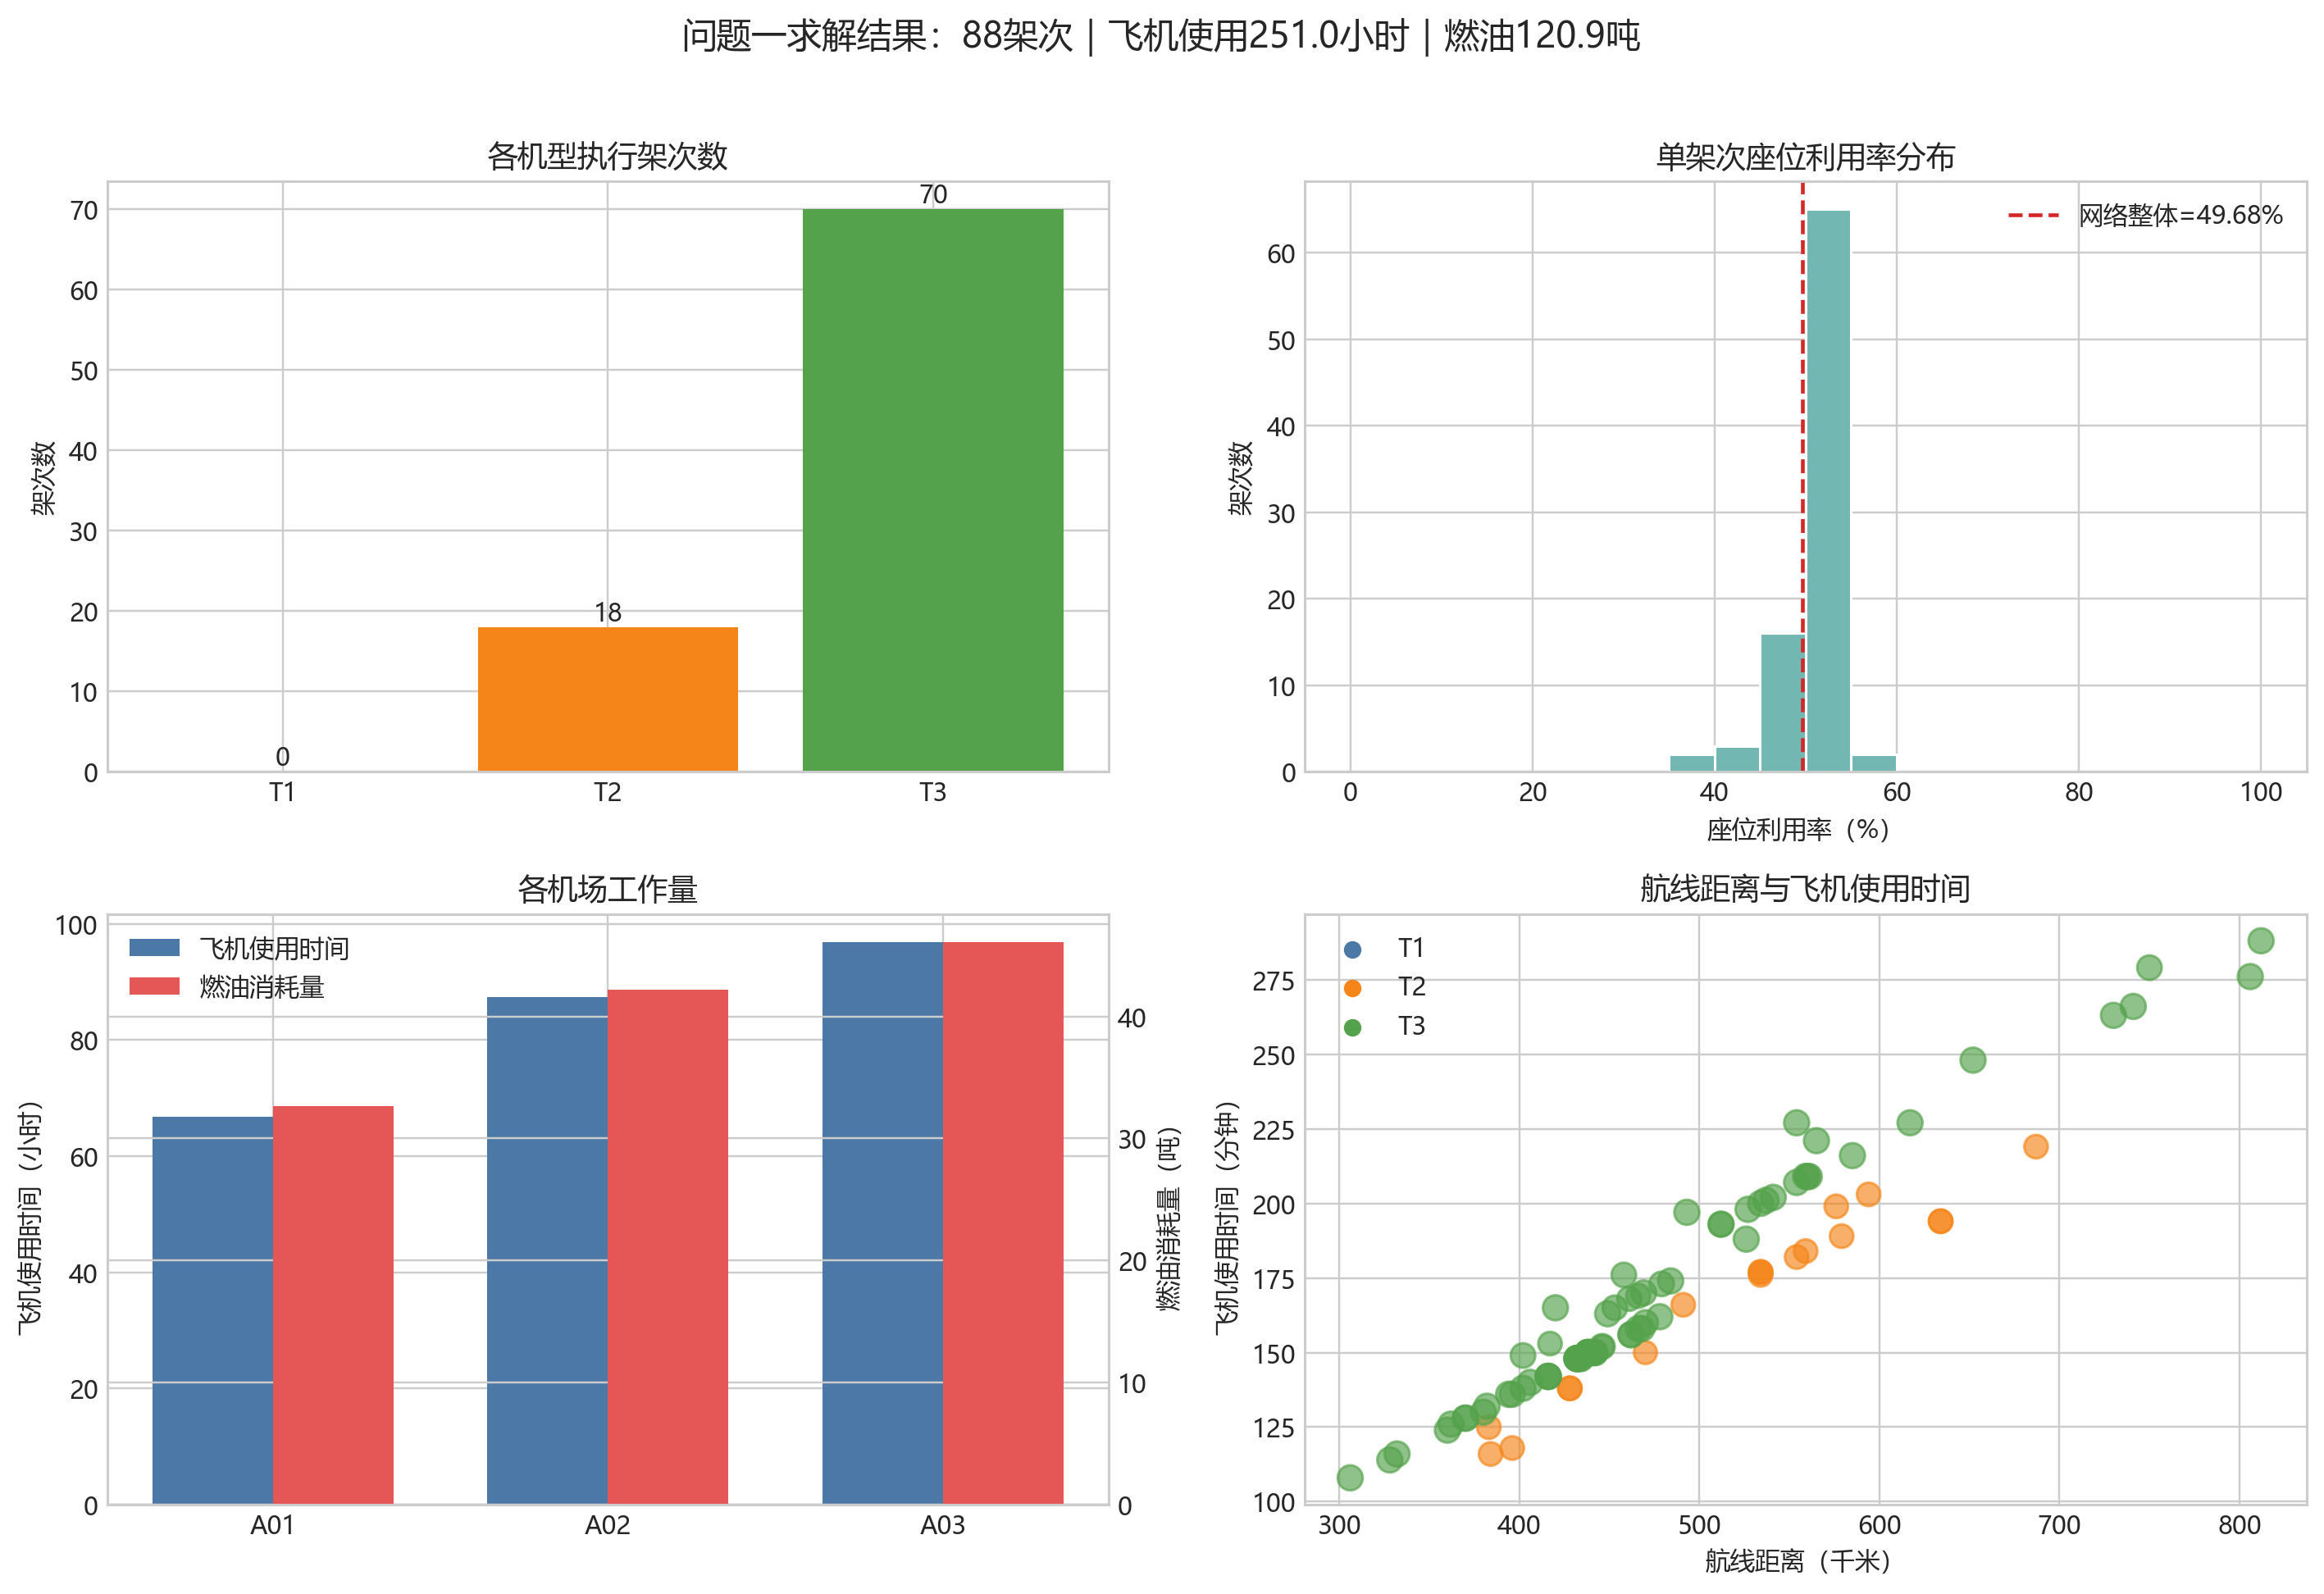
\includegraphics[width=0.72\textwidth]{问题一_求解结果综合图.png}
  \caption{问题一求解结果综合（架次结构、在途时间与利用率）}
  \label{fig:q1sum}
\end{figure}

%==================== 六、问题二 ====================
\section{问题二：出海、海返与穿梭联合运输}

\subsection{出海与海返配对、穿梭顺路承载的建模思路}

与问题一相比，问题二的本质差异在于：人员需求是包含起点终点的 OD 对，而非"送到即可"，每名人员由同一架次从起点直送终点、不换乘；载荷剖面非单调，设施上既有下机又有上机、机上人数先降后升。因此问题二属于\textbf{带同时取送的车辆路径问题}，即 VRPSPD。

通过统计问题二的数据（见表~\ref{tab:q2data}），我们得到两条关键发现：出海与海返在设施层面高度配对，穿梭均为同一区块内短途、每 OD 仅 9--19 人。受第一点启发，我们提出了"配对往返、穿梭顺路承载"的建模思路——出海与海返的满座部分配对为往返架次，去程满载送达、返程满载接回，使得架次数近乎减半；不满整座的尾数由出海、海返\textbf{各自独立}合并为环游运送。第二点则说明穿梭人数之少，环游顺路即可带走、无需单独开辟架次。由此问题二在容量结构上退化为问题一，真正新增的仅是海返与穿梭两类客流，问题一"满座 + 尾数 + 集合划分"的框架得以沿用。

\begin{table}[H]
  \centering
  \caption{问题二数据特征}
  \label{tab:q2data}
  \begin{tabular}{ll}
    \toprule
    项目 & 结论 \\
    \midrule
    需求规模 & 4000 人，出海 1600、海返 1600、穿梭 800 \\
    设施净差 $q^{\text{out}}-q^{\text{ret}}$ & 落在 $[-4,+6]$，48/52 设施在 $\pm3$ 以内 \\
    穿梭 OD & 56 对，均在同区块内短途，每 OD 9--19 人 \\
    跨机场人数 & 0，三机场解耦不产生任何损失 \\
    \bottomrule
  \end{tabular}
\end{table}

\subsection{三类需求的拆分与候选架次的构造}

\subsubsection{满座配对往返与尾数独立拆分}

出海与海返两个方向各自独立套用问题一"满座 + 尾数"拆分。满座部分：设施 $d$ 对机型 $c$ 有 $\lfloor q_d^{\text{out}}/c\rfloor$ 个出海满座与 $\lfloor q_d^{\text{ret}}/c\rfloor$ 个海返满座，因出海与海返人数接近，可配成 $\min(\lfloor q_d^{\text{out}}/c\rfloor,\lfloor q_d^{\text{ret}}/c\rfloor)$ 个往返满座加 $\big|\lfloor q_d^{\text{out}}/c\rfloor-\lfloor q_d^{\text{ret}}/c\rfloor\big|$ 个单向满座。尾数部分：出海尾数份 $\{q_d^{\text{out}}\bmod c\}$ 与海返尾数份 $\{q_d^{\text{ret}}\bmod c\}$ \textbf{各自独立、不绑定}。穿梭部分：每 OD 仅 9--19 人、不超过 19 座，不做满座拆分，作为按需部分承载量 $h_{(i,j)}\in[0,q^{\text{sh}}_{(i,j)}]$ 顺路承载。

\subsubsection{尾数合并列的组成与逐弧载荷}

一条尾数合并列 $r$ 由「机型 $m_r$ + 有向顺序 $S_r=(s_1,\dots,s_k)$ + 每站出海尾数 $d_t$、海返尾数 $p_t$，二者各自独立 + 穿梭承载 $\{h_{(i,j)}\}$」确定。设第 $t$ 站下机 $d_t$ 人、上机 $p_t$ 人，穿梭在对应两站间上下，则逐弧载荷为

\begin{equation}
  L_0=\sum_{t=1}^{k}d_t,\qquad
  L_t=\sum_{u>t} d_u+\sum_{u\le t} p_u+\sum_{i\le t<j} h_{(s_i,s_j)}\quad(t=1,\dots,k)
\end{equation}

列 $r$ 须满足四类可行条件：峰值载荷不超过座位数，即 $\max_{0\le t\le k}L_t\le c_{m_r}$；穿梭 $i$ 须在 $j$ 之前被访问；停靠次数 $k\le5$；燃油可行条件与问题一相同。其 OD 覆盖与成本为

\begin{equation}
  n_{r,(a_r,s_t)}=d_t,\quad n_{r,(s_t,a_r)}=p_t,\quad n_{r,(i,j)}=h_{(i,j)}
\end{equation}

\begin{equation}
  T_r=\frac{d_r^{\text{TSP}}}{v_{m_r}}+10k+10g_r,\qquad
  F_r=d_r^{\text{TSP}}\cdot f_{m_r},\qquad
  E_r=\sum_{\text{seg}\in r}(c_{m_r}-L_{r,\text{seg}})d_{\text{seg}}
\end{equation}

\subsection{覆盖全部出行需求的架次选择模型}

问题二中每名人员须由起点直送终点，覆盖对象从"把人送到设施"变为 OD 对；同一 OD 的人员对系统完全等价、可以互换，故按 OD 聚合人数建模、无需逐人设变量。目标仍沿分层加权结构：第一层最小化总飞机使用时间，第二层在航时最优解集内对油耗与座位利用率加权取优。

\begin{equation}
  \min\ T=\sum_{r\in\Omega} T_r\lambda_r
\end{equation}

\begin{equation}
  \text{s.t.}\quad \sum_{r\in\Omega} n_{r,(i,j)}\lambda_r=D_{(i,j)},\quad\forall(i,j)
\end{equation}

\begin{equation}
  \lambda_r\in\mathbb{Z}_+
\end{equation}

设第一层最优航时 $T^*$，第二层在航时最优解集上：

\begin{equation}
  \min\ \sum_{r\in\Omega}\Big(w_F\frac{F_r}{F_0}+w_\eta\frac{E_r}{E_0}\Big)\lambda_r
  \qquad\text{s.t.}\ \ \sum_{r\in\Omega}T_r\lambda_r=T^*,\ \ \text{式}(16)(17)
\end{equation}

其中 $F_r=d_r^{\text{TSP}}f_{m_r}$ 为列油耗、$E_r$ 为列空座$\cdot$距离，其值越小利用率越高；$F_0,E_0$ 为无量纲化基准，权重 $w_F+w_\eta=1$ 由层次分析法确定并以敏感性分析验证。与问题一的 $y_s$ 主问题不同，此处拆分约束内化到列生成中，覆盖式主问题更灵活、允许跨机型混合覆盖。

\subsection{大规模候选架次下的列生成求解}

我们首先尝试把问题一的"显式枚举 + 集合划分 IP"原样搬来。但问题二的尾数拆开使尾数份约翻倍、穿梭部分承载使选项约增至 8 倍，完整列数从问题一的数千至数万暴涨到 $10^7\sim10^8$ 量级，支撑材料中的列数探针脚本证实\textbf{预枚举不可行}。这促使我们把求解方式升级为列生成：主问题仍取集合划分形式，但不再预先生成全部列，而是维护一个只含少量列的受限主问题，以覆盖约束的对偶价为"价格信号"引导搜索、按需生成最可能改进目标的列——定价子问题不预枚举全部候选列，而是按对偶价通过 DFS 搜索生成负约化成本列。按需生成在概念上是"枚举的惰性版本"：绝大多数永远无用的列自始至终不被显式构造。

\subsubsection{列生成的两阶段总体框架}

分层加权目标决定求解分两阶段——若把加权次指标与时间固定约束并入单次列生成，第一层的最优航时无法先行确定、两目标将混叠，分成两阶段则每阶段都是标准单一目标的列生成：\textbf{阶段一}解式~(16)(17) 的 $\min T$，列生成收敛得 LP 下界，再对受限主问题 CBC 分支定界得整数最优航时 $T^*$；\textbf{阶段二}加时间固定约束 $\sum_r T_r\lambda_r=T^*$、目标换为式~(19)，重跑列生成 + CBC。每阶段内部流程相同：初始受限主问题只含满座列与每设施一条单尾数列，先解 LP 取对偶价，再由 DFS 定价子问题产生负约化成本列，迭代至无负列，最后 CBC 整数化。

\subsubsection{DFS 定价子问题与约化成本下界剪枝}

列 $r$ 的约化成本为

\begin{equation}
  \bar c_r=T_r-\sum_{(i,j)}n_{r,(i,j)}\pi_{(i,j)}
  =\frac{d_r^{\text{TSP}}}{v_{m_r}}+10k+10g_r-\sum_{t}\big(d_t\pi^{\text{out}}_{s_t}+p_t\pi^{\text{ret}}_{s_t}\big)-\sum_{(i,j)}h_{(i,j)}\pi^{\text{sh}}_{(i,j)}
\end{equation}

其中 $\pi^{\text{out}}_d,\pi^{\text{ret}}_d,\pi^{\text{sh}}_{(i,j)}$ 为出海、海返、穿梭覆盖约束的对偶价。阶段二起目标项与时间固定约束进入对偶，约化成本改写为

\begin{equation}
  \bar c_r=\Big[w_F\frac{F_r}{F_0}+w_\eta\frac{E_r}{E_0}\Big]+\lambda_0 T_r-\sum_{(i,j)}n_{r,(i,j)}\pi_{(i,j)}
\end{equation}

其中 $\lambda_0$ 为时间固定约束的对偶。定价子问题采用深度优先搜索 + 约化成本下界剪枝：枚举 $\le5$ 设施的访问顺序，逐站独立选取出海/海返尾数份与穿梭承载，当"已定部分 + 剩余下界"$\ge0$ 时回退——剩余下界取未访问部分所能取得的最乐观约化成本估计，从而保证不遗漏任何负约化成本列，又不必展开完整 $10^8$ 列空间。

\subsubsection{整数解与最优性下界}

列生成收敛处的 LP 最优给出下界 $z_{LP}$。整数解由受限主问题 CBC 分支定界求取，即"列生成 + 受限主问题 IP"而非完整 branch-and-price、不在分支节点重跑定价，故整数解是启发式上界 $z_{IP}$，最优性 gap 以 $(z_{IP}-z_{LP})/z_{LP}$ 报告，gap 小即表明整数解接近全局最优。燃油不写入主问题，在列生成阶段逐列校验/修复：相邻两停靠点间航段若超出该机型最大无加油航程，则就近插入中途加油点并同步更新 $T_r$ 与 $F_r$。

\subsection{问题二的求解结果与指标分析}

（待求解器运行后回填）总飞机使用时间 XXX 分钟、人员总在途时间 XXX 分钟、总架次数 XXX、总燃油消耗量 XXX kg、座位利用率 XX\%，与 LP 下界 gap 为 XX\%。

%==================== 七、问题三 ====================
\section{问题三：带时间要求的多日排班}

\subsection{紧核单天固定与松壳跨天可选的分层思路}

问题三在问题二路由结构不变的基础上，叠加时间窗与有限机队两重约束。沿用问题二的列生成框架是自然的起点，但"哪天飞"与"机队是否排得开"两个新问题需要一个不破坏列生成结构的处理方式。我们统计各任务类型的窗口分布（表~\ref{tab:q3data}），发现任务类型与窗口紧度高度相关，据此把需求分为紧核与松壳两层，其求解顺序与题目"应急处置 $\to$ 增储上产 $\to$ 常规倒班 $\to$ 临时任务"一致。这一划分正是后文"日级主问题 + 天内排班"两层模型的由来：主问题决定"哪天飞"并给出宽松日容量，天内 ILP 精确回答"排不排得开"。

\begin{table}[H]
  \centering
  \caption{问题三任务类型与窗口紧度}
  \label{tab:q3data}
  \begin{tabular}{lcccc}
    \toprule
    任务类型 & 人数 & 窗口时长 & 跨天数 & 层次 \\
    \midrule
    应急处置 emergency & 40 & 0.47--3.37 h & 单天 & 紧核 \\
    增储上产 production & 360 & 1.43--4.90 h & 单天 & 紧核 \\
    常规倒班 shift & 3440 & 7.3--74.8 h & $\approx2.65$ 天 & 松壳 \\
    临时任务 temporary & 160 & 32--145 h & $\approx4.1$ 天 & 松壳 \\
    \bottomrule
  \end{tabular}
\end{table}

\textbf{紧核 400 人}，即应急处置与增储上产，窗口全部落在单天内，其航班被迫落在窗日、且多设施绕行在物理上不可行，只能组织为小群组直飞/短途架次；\textbf{松壳 3600 人}，即常规倒班与临时任务，窗口跨 2--4 天，"哪天飞"是真正的决策变量。规划期 7 天、即 08-03 至 08-09，机队表~\ref{tab:fleet} 每机场 8 架，三机场已解耦、不存在跨机场争夺。

\subsection{需求到执行日的分配与时间窗刻画}

引入时间窗后，同一 OD 的人员窗口各异、不再完全可互换，因此须按 (OD, 任务类型) 进一步细分为需求类 $c=((i,j),\tau)$。若把起飞时刻直接写进列定义，每条列将携带时刻维、列数爆炸。观察数据发现：人员时间窗是连续区间、可行日集合必为连续日段，于是"能在第 $d$ 天乘列 $r$ 的人数"有上界 $D_{(i,j),d}^{\tau}$，日指派可行当且仅当"各类逐日安排人数不超过 $D_{(i,j),d}^{\tau}$、且各类总安排人数恰为 $D_{(i,j)}^{\tau}$"。据此时间窗的全部信息被压缩为逐日计数上限，问题三在 OD 聚合之上仅多一层"逐日计数"，即可把时间窗精确嵌入主问题而无需逐人建模。以"航线 $r$ + 执行日 $d$"为列：

\begin{equation}
  \min \sum_{r\in\Omega}\sum_{d\in\mathcal{D}} T_r\,\lambda_{r,d}
\end{equation}

\begin{equation}
  \text{s.t.}\quad \sum_{r\in\Omega}\sum_{d\in\mathcal{D}} n_{r,(i,j)}^{\tau}\,\lambda_{r,d} = D_{(i,j)}^{\tau},\quad \forall(i,j),\forall\tau
\end{equation}

\begin{equation}
  \sum_{r\in\Omega} n_{r,(i,j)}^{\tau}\,\lambda_{r,d} \le D_{(i,j),d}^{\tau},\quad \forall(i,j),\forall\tau,\forall d
\end{equation}

\begin{equation}
  \sum_{r:\,a_r=a} T_r\,\lambda_{r,d} \le C_{(a,d)},\quad \forall d
\end{equation}

\begin{equation}
  \lambda_{r,d}\in\mathbb{Z}_+
\end{equation}

式~(23) 保证每类需求被恰好覆盖；式~(24) 为逐日计数约束、把时间窗嵌入主问题，紧核需求据此被锁定到窗日；式~(25) 为宽松日容量，初值取 8 架飞机、14 小时运营时长，其精确可行性由天内排班保证、并通过反馈收紧。

候选列沿用问题二的满座列与尾数合并列，叠加日可行性：对列 $r$ 的每位乘客，由其时间窗与路线上到达起终点的行驶时长反解可行起飞区间，列 $r$ 在第 $d$ 天可行当且仅当全体乘客可行起飞区间之交与第 $d$ 天运营窗口相交，其中运营窗口指起飞时间在 $06{:}00$--$18{:}00$、返航不晚于 $20{:}00$；仅对可行的 $d$ 生成列 $(r,d)$。

\subsection{每日架次到飞机与时刻的精确排布}

主问题给出每个 (机场, 天) 的架次集合后，须把它们精确排到时间轴与 8 架飞机上。若把"架次落到哪架飞机、哪个时刻"也并入主问题，变量将按"架次 $\times$ 飞机 $\times$ 时刻"膨胀、且破坏列生成结构；而天内排班规模小、结构独立，故单独建时间索引 ILP 精确求解。设架次 $f$ 时长 $T_f$、机型 $m_f$、可行起飞区间 $[s_f,e_f]$，时间按步长 $\Delta$ 离散，决策变量 $x_{f,a,t}=1$ 表示架次 $f$ 由飞机 $a$ 在时刻 $t$ 起飞：

\begin{equation}
  \text{s.t.}\quad \sum_{a\in\mathcal{A}_{m_f}}\sum_{t} x_{f,a,t} = 1,\quad \forall f
\end{equation}

\begin{equation}
  x_{f,a,t}=0,\quad \forall f,a\notin\mathcal{A}_{m_f};\qquad x_{f,a,t}=0,\quad \forall f,\ t\notin[s_f,e_f]
\end{equation}

\begin{equation}
  \sum_{f}\ \sum_{t':\ t-T_f-30 < t'\le t} x_{f,a,t'} \le 1,\quad \forall a,\forall t
\end{equation}

式~(28) 每架次恰好起飞一次且只能指派给机型匹配的飞机；式~(29) 剔除机型不匹配与越出可行起飞区间的变量；式~(30) 对每架飞机、每时刻要求"已起飞且尚未完成、含 30 分钟周转"的架次至多一个，即同一飞机上的架次不重叠且满足 30 分钟周转。该 ILP 为纯 0-1 可行性问题、规模小，每机场每天约 30--40 个架次、8 架飞机、若干时隙，CBC 可精确求解。

\subsection{非临时与临时任务的两阶段编排与分层目标}

临时任务的两阶段处理直接来自题面：临时任务可因减少开销而取消，且要求先在不考虑临时任务时编排得到总时间、再在不超过该时间的条件下尽可能满足临时需求。据此：\textbf{阶段一，处理非临时需求}：主问题只含非临时需求类，式~(23) 取等号，按分层加权目标求解得总飞机使用时间 $T_0$。\textbf{阶段二，加入临时需求}：加入临时需求类，其覆盖约束式~(23) 改为"$\le$"、即可少满足，并增加预算约束

\begin{equation}
  \sum_{r\in\Omega}\sum_{d\in\mathcal{D}} T_r\,\lambda_{r,d} \le T_0
\end{equation}

阶段二目标按字典序：先最大化临时满足人数，再按加权次指标取优：

\begin{equation}
  \max \sum_{\text{temporary }(i,j)}\sum_{r,d} n_{r,(i,j)}^{\text{temporary}}\,\lambda_{r,d}
  \quad\to\quad \min \sum_{r,d}\Big[w_P\tfrac{P_r}{P_0}+w_F\tfrac{F_r}{F_0}+w_\eta\tfrac{E_r}{E_0}\Big]\lambda_{r,d}
\end{equation}

\textbf{分层加权目标贯穿两阶段}：第一层最小化总飞机使用时间、作为硬目标，第二层在航时最优解集内对人员在途时间、油耗、座位利用率加权取优：

\begin{equation}
  \min \sum_{r,d} T_r\lambda_{r,d}
  \quad\Longrightarrow\quad \min \sum_{r,d}\Big[w_P\tfrac{P_r}{P_0}+w_F\tfrac{F_r}{F_0}+w_\eta\tfrac{E_r}{E_0}\Big]\lambda_{r,d}\ \ \text{s.t.}\ \sum_{r,d}T_r\lambda_{r,d}=T^*
\end{equation}

实现上用"约束固定 + 一次重解"：先求最优总时间 $T^*$，加约束 $\sum T_r\lambda_{r,d}=T^*$ 后直接最小化加权次指标得唯一解。$P_0,F_0,E_0$ 为无量纲化基准，使分钟、千克、空座距离这三个量纲可以相加，权重 $w_P+w_F+w_\eta=1$ 由层次分析法确定并以敏感性分析验证。各列系数 $T_r,P_r,F_r,E_r$ 均为逐列常数，式~(33) 仍是 $\lambda$ 的线性整数规划。

\subsection{日级方案的高效生成与天内可排性保证}

求解沿用问题二的列生成主循环，再针对问题三新增的两个约束补上两个环节，共五步：\textbf{(1)} 三机场解耦独立求解；\textbf{(2)} 定价子问题生成列；\textbf{(3)} 日级列生成惰性加列至收敛；\textbf{(4)} 天内排班反馈收紧日容量；\textbf{(5)} 分层加权重解与两阶段。其中第 (2) 步叠加时间窗的可行日扩展、第 (4) 步解决机队资源冲突，是问题三新增的关键环节，分述如下。

\subsubsection{定价子问题与可行日扩展}

DFS 定价子问题复用问题二、叠加可行日扩展：生成列 $r$ 时反解各乘客可行起飞区间、推出可行日集合 $\mathcal{D}_r$，对每个可行日 $d\in\mathcal{D}_r$ 生成列 $(r,d)$。列规模相对问题二仅放大"平均可行天数"常数因子，松壳为 2--4 天、紧核为 1 天，量级 $10^7\sim10^8$ 级、预枚举不可行，故与问题二一致按 DFS 定价按需产列。列 $(r,d)$ 的约化成本为

\begin{equation}
  \bar c_{r,d}=T_r-\sum_{(i,j),\tau} n_{r,(i,j)}^{\tau}\big(\pi_{(i,j)}^{\tau}+\mu_{(i,j),d}^{\tau}\big)-T_r\,\alpha_{(a_r,d)}
\end{equation}

其中 $\pi_{(i,j)}^{\tau}$、$\mu_{(i,j),d}^{\tau}$、$\alpha_{(a_r,d)}$ 分别为式~(23)(24)(25) 的对偶价；与问题二相比新增的两项含义明确——逐日计数约束的对偶 $\mu$ 计入"该日覆盖"的收益、日容量约束的对偶 $\alpha$ 按架次耗时计入。进入分层加权重解后，目标系数由 $T_r$ 换为加权次指标、并叠加时间固定约束的对偶 $\lambda_0$：

\begin{equation}
  \bar c_{r,d}=\Big[w_P\tfrac{P_r}{P_0}+w_F\tfrac{F_r}{F_0}+w_\eta\tfrac{E_r}{E_0}\Big]+\lambda_0 T_r-\sum_{(i,j),\tau}n_{r,(i,j)}^{\tau}\big(\pi_{(i,j)}^{\tau}+\mu_{(i,j),d}^{\tau}\big)-T_r\,\alpha_{(a_r,d)}
\end{equation}

阶段二加入临时后，时间固定约束换为预算不等式式~(31)、其对偶 $\lambda_0\ge0$，并叠加固定临时满足人数的约束项，其余项不变。定价由 DFS 定价子问题返回最小约化成本，取 $\bar c_{r,d}<-\varepsilon$ 的列加入受限主问题，迭代至 $\min\bar c_{r,d}\ge-\varepsilon$、即 LP 收敛，随后对受限主问题分支定界求整数解，gap 以 LP 下界报告。

\subsubsection{天内可行性反馈与日容量收紧}

列生成收敛得到的是日级方案，而日容量 $C_{(a,d)}$ 只是宽松上界，不保证当天架次能在时间轴上无重叠排开，故第 (4) 步对每一机场的每一天取该日被选中的架次，用前文时间索引排班 ILP 精确判定可行性：可行则保留该日方案；不可行则回加割平面收紧 $C_{(a,d)}$ 或禁止该日特定架次组合，重解主问题，迭代至全部 21 个机场—天组合均可行。这一"主问题给出日级方案、天内 ILP 作可行性判定并回馈割平面"的循环是一种 Benders 式分解，保证最终方案一定可在天内排开，同时避免主问题内直接展开时间维导致的规模爆炸。

\subsection{问题三的求解结果与指标分析}

（待求解器运行后回填）临时人员满足 XXX 人、满足率 XX\%，总飞机使用时间 XXX 分钟、人员总在途时间 XXX 分钟、总架次数 XXX、总燃油消耗量 XXX kg、座位利用率 XX\%。

%==================== 八、模型评价与改进 ====================
\section{模型的评价与改进}

\subsection{模型的优点}

\begin{enumerate}[itemsep=2pt]
  \item \textbf{分解彻底}：利用需求按设施号段分块、架次不跨机场、机队按机场固定三条结构性事实，把三机场问题无损失解耦为三个同构子问题，规模大幅下降、可精确求解；
  \item \textbf{目标分层}：三问统一采用"第一层最小化总航时、第二层在航时最优解集内加权取优次指标"的分层加权结构，既严格贴合"在最小化总飞机使用时间的基础上优化其他因素"的题意，又保证主目标最优；
  \item \textbf{精确算法}：问题一显式枚举 + 集合划分 IP 得 gap 0.13\%；问题二、三列生成 + 受限主问题 IP，并以 LP 松弛下界客观评估解质量；
  \item \textbf{层次递进}：问题三把时间窗精确嵌入"逐日计数"、以"紧核单天固定、松壳跨天可选"结构把难题化为与优先级一致的求解顺序。
\end{enumerate}

\subsection{模型的不足与改进方向}

\begin{enumerate}[itemsep=2pt]
  \item \textbf{LAND 分配的固定}：问题一将 LAND 乘客按设施分块固定归属机场，当不同机场到同一设施距离差异显著时可能非最优。更精细的做法是把 LAND 分配纳入决策，引入整数变量 $z_{d,a}$，表示设施 $d$ 的 LAND 乘客分给机场 $a$ 的人数，与 $\min\sum_a\mathrm{VSP}(a)$ 合并为整体 IP，此时三机场通过 $z_{d,a}$ 耦合、需采用列生成与分支定价；
  \item \textbf{拆分粒度的残差}：机型感知拆分把尾数份视为原子，例如 $q=29$ 取 T2 得尾数 13，不能再拆成 $10+3$ 去搭不同架次的便车，这损失了"尾数份二次拆分"的合并自由度，但二次拆分通常多出一个架次、影响很小；若需完全灵活可回到"1 人份 + 列生成"的精细框架；
  \item \textbf{整数解的近似性}：问题二、三的整数解由受限主问题分支定界给出，非完整 branch-and-price，是最优性 gap 可报告的启发式上界；若需更强最优性保证可完整实现分支定价；
  \item \textbf{天内排班的离散近似}：时间索引 ILP 以步长 $\Delta$ 离散时刻，步长越小越精确但变量越多，需在精度与规模间折中。
\end{enumerate}

%==================== AI 工具使用声明 ====================
\section*{AI 工具使用声明}

本参赛队在竞赛过程中使用了 AI 工具，主要用于语言润色、公式整理与代码调试辅助，详细使用情况见支撑材料。

%==================== 参考文献 ====================
\section*{参考文献}

\begin{thebibliography}{9}
\bibitem{ref:toth} Toth P, Vigo D. Vehicle Routing: Problems, Methods, and Applications (2nd ed.)[M]. Philadelphia: SIAM, 2014.
\bibitem{ref:cg} L{\"u}bbecke M E, Desrosiers J. Selected topics in column generation[J]. Operations Research, 2005, 53(6): 1007--1023.
\bibitem{ref:primer} Desrosiers J, L{\"u}bbecke M E. A primer in column generation[M]//Column Generation. Boston: Springer, 2005: 1--32.
\bibitem{ref:sd} Archetti C, Speranza M G. Vehicle routing problems with split deliveries[J]. International Transactions in Operational Research, 2012, 19(1-2): 3--22.
\bibitem{ref:ilp} 整数线性规划(ILP)方法[EB/OL]. \url{https://blog.csdn.net/zouxiaolv/article/details/88835878}.
\end{thebibliography}

%==================== 附录 ====================
\appendix
\section{支撑材料文件列表}

\begin{enumerate}[itemsep=1pt]
  \item 数据文件：\texttt{distances.csv}、\texttt{peopleQ1.csv}、\texttt{peopleQ2.csv}、\texttt{peopleQ3.csv}（赛题提供）；
  \item 结果文件：\texttt{q1-routes.csv}、\texttt{q1-assignments.csv}（问题一已求解），\texttt{q2-*}、\texttt{q3-*}（待回填）；
  \item 求解程序：\texttt{code/q1\_solver.py}（问题一求解器），\texttt{code/列数探针.py}、\texttt{code/探针Q1.py}、\texttt{code/探针Q2.py}、\texttt{code/探针Q2\_full.py}（列规模探针），\texttt{code/统计请求.py}、\texttt{code/热力图.py}（数据统计与可视化）；
  \item 可视化：\texttt{output/问题一\_航线网络图.png}、\texttt{output/问题一\_求解结果综合图.png}、\texttt{output/question1\_OD矩阵热力图.png}、\texttt{output/question2\_OD矩阵热力图.png}；
  \item AI 工具使用详情：\texttt{AI 工具使用详情.pdf}。
\end{enumerate}

\section{问题一求解程序源代码}

问题一的完整可运行源程序见支撑材料 \texttt{code/q1\_solver.py}，其核心为"尾数合并架次枚举 + 集合划分整数规划 + 燃油后置校验"：

\lstinputlisting[language=Python, caption={问题一求解器 q1\_solver.py}]{../code/q1_solver.py}

\end{document}
